\documentclass{article}

\usepackage[nonatbib, final]{neurips}
\usepackage[numbers,sort&compress]{natbib}

\makeatletter
\renewcommand{\@noticestring}{\centering}
\makeatother

\input{extra_pkgs}

\usepackage{amsmath}
\usepackage{amssymb}
\usepackage{multirow}
\usepackage{tikz}
\usetikzlibrary{arrows.meta,positioning,fit,shapes.geometric}

\newcommand{\method}{Relation-Grounded Floor Repair}
\newcommand{\fp}{Floor-Prior}
\newcommand{\eg}{e.g.,\ }
\newcommand{\ie}{i.e.,\ }

\title{Repairing Graph-to-Layout Relation Grounding in Instruction-Guided 3D Indoor Scene Generation}

\author{
  Anonymous Authors \\
  Anonymous Institution \\
  \texttt{anonymous@example.com}
}

\begin{document}

\maketitle

\begin{abstract}
Instruction-guided 3D indoor scene generation requires final layouts to realize the spatial relations requested by a user, not merely to generate plausible object sets or symbolic scene graphs. We show that a pretrained InstructScene pipeline exhibits a graph-to-layout grounding gap: explicit relations in the instruction can be lost when a generated scene graph is decoded into continuous object placements. We introduce \method, a training-free, safety-aware verifier-repair framework that parses explicit spatial relations, matches them to generated objects, verifies whether final layouts satisfy them, and applies bounded floor-plane repairs while preserving object height. On the existing InstructScene bedroom, living-room, and dining-room validation splits, the collision-gated \fp{} repair improves realized relation accuracy by 7.8, 8.8, and 7.8 absolute points, respectively, with a weighted gain of 8.2 points. The same gated variant reduces FCL mesh-collision pair rates below the baseline. These results support final-layout relation grounding as a lightweight and reproducible path toward more instruction-faithful 3D indoor scene synthesis.
\end{abstract}

\section{Introduction}

Text-conditioned 3D indoor scene generation is useful for embodied AI, simulation, game production, and interactive design. In these settings, spatial language is not decorative. If a prompt asks for a nightstand behind a bed or a coffee table to the right of a side table, the generated layout must realize that relation in geometry. Recent indoor scene generators synthesize plausible object arrangements from scene categories, floor plans, scene graphs, or text~\citep{paschalidou2021atiss,wang2021sceneformer,tang2024diffuscene,lin2024instructscene}. However, a symbolic relation that appears in an intermediate graph does not guarantee that the final continuous layout satisfies the requested relation.

This paper studies this failure mode in InstructScene~\citep{lin2024instructscene}, an instruction-driven 3D indoor scene synthesis pipeline with a semantic graph prior. We identify a \emph{graph-to-layout grounding gap}: an instruction may contain explicit spatial relations, and the generator may produce plausible scenes, yet the decoded object centers can violate the requested relations. Rather than train a new generator or introduce a new benchmark, we ask whether a lightweight verifier-repair layer can improve relation realization using the existing InstructScene checkpoints, validation prompts, and evaluation protocol.

We propose \method, a plug-in final-layout relation grounding module. Given a generated layout and its source instruction, the module extracts explicit spatial relation triples, matches the triples to generated object categories, verifies whether the floor-plane geometry satisfies them, and repairs object translations when a relation is violated. The final design repairs only the horizontal floor plane, preserving the vertical coordinate of every object. This detail matters in practice: early 3D repair variants can improve relation metrics while producing visually implausible scenes with floating furniture. Our \fp{} variant selects among bounded candidate repairs using relation satisfaction and overlap-aware scoring, and a collision-gated verifier can fall back to the baseline layout whenever mesh collision increases.

Our experiments use the original InstructScene bedroom, living-room, and dining-room validation splits. The main collision-gated \fp{} repair improves realized relation accuracy from 0.739 to 0.816 in bedrooms, 0.551 to 0.639 in living rooms, and 0.595 to 0.673 in dining rooms, with absolute gains of +7.76, +8.84, and +7.81 points and a weighted gain of +8.2 points. Ungated \fp{} and direct repair variants are retained as diagnostic ablations: they can obtain larger relation gains, but the paper-facing main method uses collision gating because it preserves the mesh-validity claim. Across three seeds, relation gains remain positive for all room types after collision gating, while mean mesh-collision pair deltas become negative. Real 3D-FUTURE mesh render diagnostics show selected \fp{} examples improve relation counts without increasing mesh pairs and with high before/after structural similarity.

Our contribution is not a claim of first relation-aware 3D scene generation, nor a claim that a post-generation layer replaces stronger full generators. Strong related systems use scene graphs, semantic dependency graphs, language models, and optimization to reason about spatial constraints~\citep{feng2023layoutgpt,yang2024holodeck,zhai2023commonscenes,bucher2026respace,gao2026sdgscenes}. Instead, this paper makes a narrower and reproducible claim:
\begin{itemize}[leftmargin=1.5em]
    \item We identify and quantify a graph-to-layout grounding gap in an existing instruction-guided 3D scene generator.
    \item We introduce a training-free relation-grounded post-generation control framework: relation parsing, object matching, geometric verification, bounded floor-plane repair, and collision-gated validation.
    \item We show that safety-aware repair---height preservation, movement bounds, and mesh-collision gating---provides a safer paper-facing method than direct relation repair alone.
\end{itemize}

\begin{figure}[t]
\centering
\resizebox{0.98\linewidth}{!}{
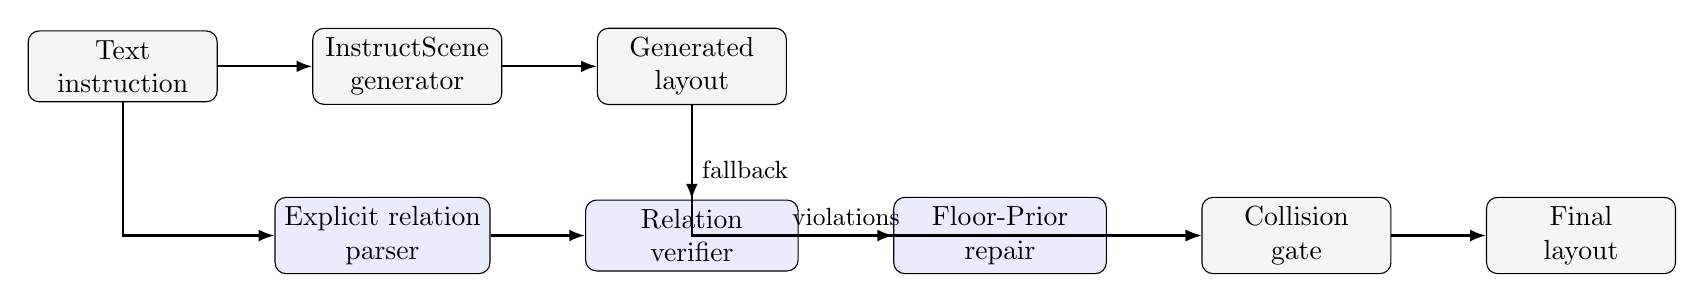
\begin{tikzpicture}[
  node distance=1.2cm,
  block/.style={draw, rounded corners, align=center, minimum width=2.4cm, minimum height=0.9cm, fill=gray!8},
  ours/.style={draw, rounded corners, align=center, minimum width=2.7cm, minimum height=0.9cm, fill=blue!8},
  arrow/.style={-{Latex[length=2mm]}, thick}
]
\node[block] (prompt) {Text\\instruction};
\node[block, right=of prompt] (gen) {InstructScene\\generator};
\node[block, right=of gen] (layout) {Generated\\layout};
\node[ours, below=of layout] (verify) {Relation\\verifier};
\node[ours, left=of verify] (parse) {Explicit relation\\parser};
\node[ours, right=of verify] (repair) {\fp{}\\repair};
\node[block, right=of repair] (gate) {Collision\\gate};
\node[block, right=of gate] (out) {Final\\layout};
\draw[arrow] (prompt) -- (gen);
\draw[arrow] (gen) -- (layout);
\draw[arrow] (prompt) |- (parse);
\draw[arrow] (layout) -- (verify);
\draw[arrow] (parse) -- (verify);
\draw[arrow] (verify) -- node[above, font=\small]{violations} (repair);
\draw[arrow] (repair) -- (gate);
\draw[arrow] (layout) |- node[pos=0.25, right, font=\small]{fallback} (gate);
\draw[arrow] (gate) -- (out);
\end{tikzpicture}}
\caption{\textbf{\method{} overview.} We keep the pretrained InstructScene generator fixed, parse explicit spatial relations from the input instruction, match them to generated objects, verify the final continuous layout, and repair violated relations in the floor plane while preserving object height. The collision gate falls back to the original layout when mesh collision would increase.}
\label{fig:overview}
\end{figure}

\section{Related Work}

\paragraph{Indoor scene synthesis.}
3D-FRONT~\citep{fu20213dfront} and 3D-FUTURE~\citep{fu20203dfuture} provide large-scale room layouts and textured furniture assets that underpin much recent indoor scene synthesis work. ATISS~\citep{paschalidou2021atiss} models indoor scenes as unordered sets generated autoregressively. SceneFormer~\citep{wang2021sceneformer} uses transformers to generate indoor scenes conditioned on room layouts. DiffuScene~\citep{tang2024diffuscene} uses denoising diffusion over unordered object attributes. These methods focus on plausible and diverse indoor layouts; our work focuses on whether explicit natural-language relations are realized in the final layout of an instruction-conditioned pipeline.

\paragraph{Text and graph conditioned scene generation.}
InstructScene~\citep{lin2024instructscene} is our direct baseline because it synthesizes 3D indoor scenes from natural language instructions with a semantic graph prior. CommonScenes~\citep{zhai2023commonscenes} converts scene graphs into commonsense 3D scenes with scene graph diffusion. LayoutGPT~\citep{feng2023layoutgpt} uses large language models as visual planners for layouts, including spatial and numerical constraints. Holodeck~\citep{yang2024holodeck} uses language models and 3D assets to generate embodied AI environments, including spatial constraints for object placement. These works show that language and structured relations are useful interfaces for scene generation. Our contribution is complementary: we evaluate and repair the final realized relation after a pretrained instruction-to-scene pipeline has produced a layout.

\paragraph{Strong relation-aware systems.}
ReSpace~\citep{bucher2026respace} is a close text-driven indoor scene synthesis and editing framework based on structured scene representations and a specialized language model. SDGScenes~\citep{gao2026sdgscenes} uses a semantic dependency graph, VLM-derived commonsense constraints, and nonlinear constrained optimization to align scenes with user intent. These systems overlap with the broad goal of relation- and intent-aware 3D generation. We therefore do not claim to outperform them or to be the first relation-aware method. Our current fair comparison is the original InstructScene output under the same validation prompts and checkpoints; ReSpace and SDGScenes require a shared protocol before direct numerical claims are appropriate. Put differently, we do not replace strong generators; we study a plug-in final-layout relation grounding layer for an existing instruction-guided generator.

\section{Method}

\subsection{Problem Setup}

Let an instruction-conditioned generator produce a scene layout
\[
  S = \{(c_i, t_i, s_i, r_i, m_i)\}_{i=1}^{N},
\]
where object $i$ has category $c_i$, translation $t_i \in \mathbb{R}^{3}$, size $s_i$, yaw rotation $r_i$, and optionally a retrieved mesh identifier $m_i$. The instruction text $x$ contains a set of explicit spatial relations
\[
  R(x) = \{(c_a, p, c_b)\},
\]
where predicate $p$ may be left-of, right-of, in-front-of, behind, near, or far. The goal is to produce a repaired layout $S'$ that improves the realized satisfaction of $R(x)$ while preserving scene plausibility.

\subsection{Explicit Relation Extraction and Matching}

We use a deliberately simple rule-based parser to extract explicit spatial phrases. This choice makes the method transparent and keeps the benchmark unchanged. The parser output is noisy, but it is sufficient to drive a verifier: the deployable parsed-relation repair captures most of the oracle-repair gain in earlier diagnostics. The parser is not intended to solve implicit commonsense reasoning; prompts that require latent affordance or support reasoning are outside the current claim.

For each parsed triple, the verifier finds generated objects whose class labels match the subject and object categories. When multiple instances match, the verifier selects the nearest pair in the floor plane. All distance and direction checks use the $x/z$ plane; the $y$ axis is treated as vertical height.

\subsection{Relation Verification}

For a candidate object pair $(i,j)$ and predicate $p$, the verifier evaluates whether the floor-plane displacement $\Delta_{ij}=(t_i^x-t_j^x, t_i^z-t_j^z)$ satisfies the predicate. Directional predicates check the dominant signed displacement along the relevant axis; distance predicates compare floor-plane distance against close or far thresholds. We report exact selected-relation accuracy, counting a relation correct only when the target relation appears in the realized relation set.

\subsection{Direct Height-Preserving Repair}

The direct repair baseline moves an object in the floor plane to satisfy a violated relation. It preserves the original height coordinate:
\[
  t_i' = (t_i^x + \delta_x, \; t_i^y, \; t_i^z + \delta_z).
\]
This repair gives large relation gains but may move objects substantially. In our experiments, direct repair increases relation accuracy by up to 19.7 points, but average repair movement is about two meters and mesh collision can increase slightly. We therefore use direct height-preserving repair as an internal ablation, not as the main method.

\subsection{Floor-Prior Repair}

The \fp{} repair constrains relation repair with scene priors. For a violated relation, the method proposes candidate translations with interpolation strengths $\alpha \in \{0.25,0.5,0.75,1.0\}$, clamps movement by a maximum radius, and scores candidates by relation satisfaction and coarse overlap penalties. The chosen candidate must improve the relation while keeping the motion bounded. In all variants, the vertical coordinate remains unchanged.

\begin{algorithm}[t]
\caption{\fp{} relation repair}
\label{alg:floor-prior}
\DontPrintSemicolon
\KwIn{Layout $S$, parsed relations $R(x)$, thresholds $d_{\mathrm{close}}, d_{\mathrm{far}}$, max movement $\rho$, passes $K$}
\KwOut{Repaired layout $S'$}
$S' \leftarrow S$\;
\For{$k=1$ \KwTo $K$}{
  \ForEach{$(c_a,p,c_b) \in R(x)$}{
    $(i,j) \leftarrow$ nearest matching object pair in the $x/z$ plane\;
    \If{$p$ is already satisfied by $(i,j)$}{continue}
    $\mathcal{C} \leftarrow$ bounded floor-plane candidate translations for object $i$\;
    Score each $c \in \mathcal{C}$ by relation satisfaction and overlap penalty\;
    Apply the best candidate, preserving $t_i^y$\;
  }
}
\Return{$S'$}\;
\end{algorithm}

\subsection{Collision-Gated Selection}

For mesh-aware evaluation, we load the retrieved 3D-FUTURE meshes and compute FCL mesh-collision pair counts using a trimesh collision manager. The collision-gated variant keeps the repaired scene only when the repaired mesh collision pair count does not exceed the baseline count; otherwise it falls back to the baseline layout for that scene. This gate is a verifier-selection layer and should be described explicitly.

\section{Experiments}

\subsection{Experimental Setup}

We evaluate on the existing InstructScene validation splits for bedrooms, living rooms, and dining rooms. We use the official pretrained SG diffusion VQ object-feature checkpoints: bedroom epoch 1999, living-room epoch 1459, and dining-room epoch 1239. We do not create a new benchmark or add new annotations. Metrics include realized relation accuracy, average repair movement in the floor plane, mesh collision pair rate, collision-gated relation accuracy, and height-change diagnostics. For visual diagnostics, we render real 3D-FUTURE meshes for selected examples and compute CLIP text-image similarity deltas and structural similarity (SSIM) between before/after renders.

\subsection{Main Results}

Table~\ref{tab:main} compares the original InstructScene layout with the paper-facing collision-gated \fp{} repair. This main method improves relation realization in all three room categories, with gains of +7.76, +8.84, and +7.81 absolute points for bedrooms, living rooms, and dining rooms, respectively. Its weighted relation accuracy is 70.4\%, a +8.2 point improvement over the baseline, while mesh-collision pair rates are lower than the original layouts.

\begin{table}[t]
\centering
\caption{Main collision-gated \fp{} relation results. Accuracy is exact realized selected-relation accuracy; the gated variant keeps repaired layouts only when FCL mesh collision pairs do not increase.}
\label{tab:main}
\begin{tabular}{lccccc}
\toprule
Room & Baseline & Gated \fp{} & Gain & Base mesh & Gated mesh \\
\midrule
Bedroom & 0.7388 & 0.8163 & +0.0776 & 0.0702 & 0.0683 \\
Living room & 0.5510 & 0.6395 & +0.0884 & 0.0313 & 0.0310 \\
Dining room & 0.5948 & 0.6729 & +0.0781 & 0.0342 & 0.0336 \\
\bottomrule
\end{tabular}
\end{table}

For completeness, Table~\ref{tab:ungated} reports the ungated \fp{} diagnostic result. It shows the upper relation-gain direction of the floor-prior repair before collision gating, but it is not the main paper result because its mesh-collision pair delta is slightly positive.

\begin{table}[t]
\centering
\caption{Ungated \fp{} diagnostic result. These values are retained as an ablation rather than the main result.}
\label{tab:ungated}
\begin{tabular}{lccccc}
\toprule
Room & Baseline & Ungated \fp{} & Gain & Move & Mesh $\Delta$ \\
\midrule
Bedroom & 0.7388 & 0.8408 & +0.1020 & 0.7837 & +0.0029 \\
Dining room & 0.5948 & 0.7286 & +0.1338 & 0.7315 & +0.0008 \\
Living room & 0.5510 & 0.6939 & +0.1429 & 0.8808 & +0.0008 \\
\bottomrule
\end{tabular}
\end{table}

\subsection{Direct Repair Is Strong but Too Aggressive}

Table~\ref{tab:direct} shows that direct height-preserving repair achieves larger relation gains than \fp{} repair, but with substantially larger movements. This result motivates the floor-prior design: a paper-facing method should not win relation accuracy merely by pushing furniture far across the room.

\begin{table}[t]
\centering
\caption{Direct height-preserving repair. Direct repair is a strong internal baseline but moves objects much more than \fp{} repair.}
\label{tab:direct}
\begin{tabular}{lccccc}
\toprule
Room & Baseline & Direct & Gain & Move & Mesh $\Delta$ \\
\midrule
Bedroom & 0.7388 & 0.8735 & +0.1347 & 2.2101 & +0.0034 \\
Dining room & 0.5948 & 0.7844 & +0.1896 & 1.9694 & +0.0019 \\
Living room & 0.5510 & 0.7483 & +0.1973 & 2.2834 & +0.0004 \\
\bottomrule
\end{tabular}
\end{table}

\subsection{Collision-Gated Results}

Table~\ref{tab:gated} expands the conservative collision-gated \fp{} result with the ungated repair column and fallback counts. The gate reduces relation gains relative to ungated repair because it falls back on scenes where mesh collision would increase. Nevertheless, gated relation gains remain positive in every room, and gated mesh pair rates fall below baseline. This is the safest variant for mesh-validity claims and is the main method used in Table~\ref{tab:main}.

\begin{table}[t]
\centering
\caption{Collision-gated \fp{} results. The gate keeps repaired layouts only when FCL mesh collision pairs do not increase.}
\label{tab:gated}
\small
\begin{tabular}{lccccccc}
\toprule
Room & Base & Repair & Gated & Gated gain & Base mesh & Gated mesh & Fallback \\
\midrule
Bedroom & 0.7388 & 0.8408 & 0.8163 & +0.0776 & 0.0702 & 0.0683 & 6 \\
Dining room & 0.5948 & 0.7286 & 0.6729 & +0.0781 & 0.0342 & 0.0336 & 15 \\
Living room & 0.5510 & 0.6939 & 0.6395 & +0.0884 & 0.0313 & 0.0310 & 14 \\
\bottomrule
\end{tabular}
\end{table}

\subsection{Multi-Seed Stability}

Table~\ref{tab:multiseed} summarizes three-seed results for the selected \fp{} configuration before and after collision gating. Ungated relation gains are stable and positive across all rooms. After collision gating, relation gains remain positive, and the mean mesh delta is negative for every room.

\begin{table}[t]
\centering
\caption{Three-seed stability. Standard deviations are population standard deviations over three seeds.}
\label{tab:multiseed}
\begin{tabular}{lccccc}
\toprule
Room & Mean gain & Std & Mean gated gain & Gated std & Mean gated mesh $\Delta$ \\
\midrule
Bedroom & +0.1061 & 0.0058 & +0.0803 & 0.0069 & -0.0020 \\
Dining room & +0.1462 & 0.0093 & +0.0867 & 0.0098 & -0.0008 \\
Living room & +0.1270 & 0.0125 & +0.0703 & 0.0153 & -0.0003 \\
\bottomrule
\end{tabular}
\end{table}

\subsection{Movement Ablation}

A conservative movement radius of 0.8 meters reduces average movement to 0.38--0.42 meters but also reduces relation gains to 5.7--7.8 points. The main 1.8-meter setting gives a better relation-control tradeoff, while the 0.8-meter variant is useful when minimal movement is more important than maximum relation satisfaction.

\begin{table}[t]
\centering
\caption{Conservative max-move ablation. Smaller movement budgets reduce geometry changes but also reduce relation gains.}
\label{tab:maxmove}
\begin{tabular}{lcccc}
\toprule
Room & Baseline & Max 0.8 repair & Gain & Move \\
\midrule
Bedroom & 0.7388 & 0.7959 & +0.0571 & 0.4233 \\
Dining room & 0.5948 & 0.6729 & +0.0781 & 0.3881 \\
Living room & 0.5510 & 0.6156 & +0.0646 & 0.3797 \\
\bottomrule
\end{tabular}
\end{table}

\subsection{Height Preservation and Visual Diagnostics}

The height diagnostic reports $y$-changed rate 0.0 and maximum absolute $y$ delta 0.0 for the evaluated \fp{} variants. Thus the final repair does not move furniture vertically. This fixes a practical failure observed in early visualizations where chairs or sofas could appear to float.

We also rendered real 3D-FUTURE mesh comparisons. Table~\ref{tab:visual} compares the old three-example direct showcase with the new 15-example \fp{} showcase selected for relation improvement without mesh-pair increase. The \fp{} showcase has higher mean relation gain, lower mesh pair count, slightly positive CLIP delta, and high SSIM. We interpret these diagnostics conservatively: they support that selected examples do not show obvious visual degradation, but they do not prove universal human-perceived visual improvement.

\begin{table}[t]
\centering
\caption{Real-mesh visual diagnostics. CLIP delta is after-minus-before text-image similarity; SSIM measures before/after structural similarity.}
\label{tab:visual}
\begin{tabular}{lccccc}
\toprule
Showcase & Examples & Relation gain & Mesh-pair $\Delta$ & CLIP $\Delta$ & SSIM \\
\midrule
Direct y-fixed & 3 & +1.333 & 0.000 & -0.0165 & 0.8358 \\
\fp{} & 15 & +1.400 & -0.267 & +0.0027 & 0.9065 \\
\bottomrule
\end{tabular}
\end{table}

\subsection{Strong Baseline Feasibility and Missing Controls}

The feedback cycle identified three reviewer-facing controls that should be added before treating this as a main-conference submission: a random/local-move control under the same movement budget, a generic constraint-optimization repair baseline, and an oracle-parser upper bound under the final \fp{} protocol. The only fully fair same-protocol baseline currently available is the original InstructScene output. Direct y-fixed repair, \fp{} repair, and collision-gated repair are fair internal baselines and ablations because they operate on the same generated outputs and evaluation splits. ReSpace and SDGScenes are strong related systems, but no same-split shared-protocol reproduction has been completed. ReSpace requires its own SSR-3DFRONT protocol, separate environment, vLLM and model access; SDGScenes has no verified same-split runnable path on our server. We therefore cite these methods as close related work and avoid outperforming claims.

\section{Discussion}

The results support a narrow but useful conclusion: relation-aware post-generation control can substantially improve explicit spatial relation realization in an existing instruction-guided scene generator. The difference between direct repair and \fp{} repair is important. Direct repair shows the upper effect size of simple geometric relation correction, but it is too aggressive for a polished method. \fp{} repair gives smaller but still substantial gains with bounded movement, unchanged object heights, and collision-gated validity control.

The results also reveal an evaluation lesson. Reporting only symbolic scene graph correctness can miss failures in the final continuous layout. Conversely, reporting only visual examples can hide whether the requested relation is actually satisfied. A relation-aware scene generation benchmark should evaluate instruction parsing, graph-level relation accuracy, final layout relation accuracy, and geometric side effects separately.

\section{Limitations}

The current method targets explicit spatial relations. It does not handle all implicit commonsense requirements, such as affordance, reachability, support, or task-specific functional arrangements. The parser is rule-based and intentionally simple; stronger language parsing may further improve recall and precision. The collision-gated variant is a post-hoc verifier-selection layer, not an end-to-end collision-aware generator. Our visual diagnostics use selected examples, CLIP similarity, SSIM, and mesh-pair counts; they are not a substitute for a human preference study. Finally, we do not claim superiority over ReSpace, SDGScenes, or other strong related methods without a shared evaluation protocol.

\section{Conclusion}

We presented \method, a training-free verifier-repair layer for instruction-guided 3D indoor scene generation. The method addresses a graph-to-layout grounding gap in InstructScene by parsing explicit spatial relations, verifying final layout geometry, and applying bounded floor-plane repairs that preserve object heights. On existing InstructScene validation splits, \fp{} repair consistently improves realized relation accuracy, while collision-gated variants retain positive gains and control FCL mesh collision. These results make relation-consistency repair a practical and reproducible direction for improving pretrained 3D scene generators.

\section*{Reproducibility Notes}

All reported data are archived locally under \texttt{experiment\_archive/}\\
\texttt{relation\_aware\_instructscene\_20260530}. The archive contains remote raw evaluation JSON/TXT files, local result tables, rendered visual assets, analysis scripts, documentation, a manifest, and SHA256 checksums. Raw datasets, checkpoints, and environments are excluded because they are large third-party assets.

\bibliographystyle{plainnat}
\bibliography{references}

\appendix

\section{Additional Result Tables}

\begin{table}[h]
\centering
\caption{Key archived tables used in this draft.}
\label{tab:archive}
\begin{tabular}{lcc}
\toprule
Table & Rows & Columns \\
\midrule
\texttt{floor\_prior\_results.csv} & 33 & 15 \\
\texttt{floor\_prior\_gated\_results.csv} & 33 & 14 \\
\texttt{floor\_prior\_mesh\_results.csv} & 33 & 11 \\
\texttt{visual\_quality\_real\_mesh.csv} & 18 & 31 \\
\texttt{strong\_baseline\_feasibility.csv} & 6 & 7 \\
\bottomrule
\end{tabular}
\end{table}

\section{NeurIPS Checklist Placeholder}

This is a first draft. A complete NeurIPS checklist should be filled before submission, including compute resources, statistical methodology, dataset licenses, artifact release plans, and limitations.

\end{document}
